\section{Pulse sequences}
\label{sec:theory__pulse_sequences}

It is impossible to provide a full overview of all, or even most, of the major NMR experiments in widespread use; the reader is directed to other books for this purpose.\autociteset{textbooks-experiments}
I seek only to (briefly) explain the general structure of one- and two-dimensional Fourier transform experiments, and in particular, how the formalisms developed in previous sections can be used to analyse and simulate such experiments.

\subsection{1D pulse--acquire}
\label{subsec:theory__pulseacq}

Consider the simplest NMR experiment, a 1D \proton{} pulse--acquire spectrum (\cref{fig:pulse_acquire}).
This consists of a \ang{90} pulse, immediately followed by detection; for convenience, we will first consider the pulse as being applied along the $+y$-axis, i.e. with a phase of $\phi = \pi/2$.

\begin{figure}[htbp]
    \centering
    \label{fig:pulse_acquire}
    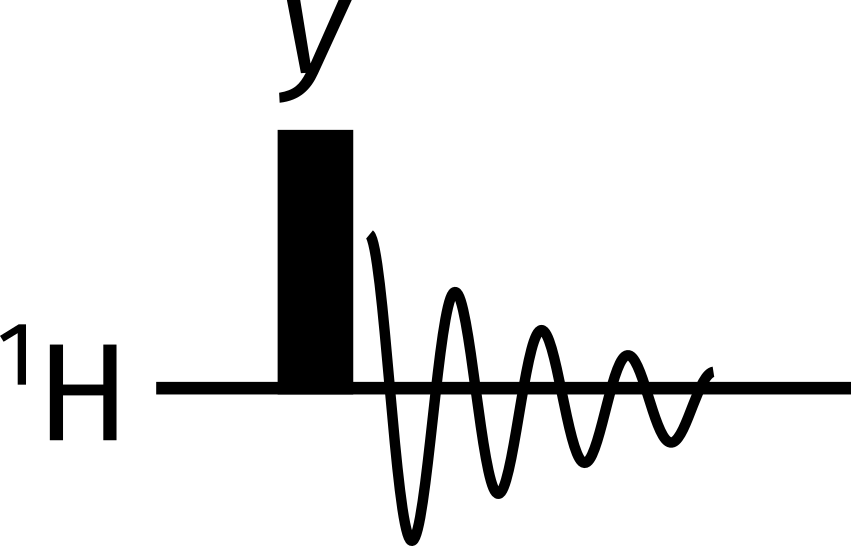
\includegraphics[]{pp/zg_y.png}%
    \caption[Pulse--acquire experiment]{1D \proton{} pulse--acquire experiment.}
\end{figure}

To understand this, we begin with the thermal density operator $\rho_0' = I_z$ (\cref{eq:rho0_simplified}) and assume that there is only one spin in the sample, and that the pulse is applied on-resonance.
The corresponding Hamiltonian during the pulse is simply $\omega_1 I_y$ (\cref{eq:hard_pulse_onresonance}).
If the duration of the pulse is $\taup$, then the density operator immediately following the pulse is given by:
\begin{equation}
    \label{eq:rho_after_pulse}
    \rho = \exp(-\mi\omega_1 I_y\taup) I_z \exp(\mi\omega_1 I_y\taup) = \cos(\omega_1\taup)I_z + \sin(\omega_1\taup)I_x.
\end{equation}
In this case, to obtain a \ang{90} pulse, $\taup$ is specifically calibrated to ensure that $\omega_1\taup = \pi/2$, which yields
\begin{equation}
    \label{eq:rho_after_pulse_simplified}
    \rho = I_x.
\end{equation}
During the detection period, this term evolves under $H_\text{free} = H_\text{cs} = \omega_0 I_z$.
(We use the Schr\"odinger-picture free Hamiltonian here because the measurement of the NMR signal takes place in the laboratory frame.)
At a time $t$ after detection has begun, the density operator is thus:
\begin{equation}
    \label{eq:rho_during_detection}
    \rho(t) = \exp(-\mi \omega_0 I_z t)I_x\exp(\mi\omega_0 I_z t) = \cos(\omega_0 t)I_x + \sin(\omega_0 t)I_y.
\end{equation}
The NMR signal derives from both $x$- and $y$-magnetisation ($M_x$ and $M_y$), which are in turn proportional to $I_x$ and $I_y$ by a factor of $\gamma$.
(If multiple spins are present, then each spin induces its own magnetisation: we would have that $M_x = \sum_i \gamma_i I_{ix}$, and likewise for $M_y$.)
These are then combined to form a complex signal (this process is known as \textit{quadrature detection}):
\begin{align}
    s(t) &= M_x(t) + \mi M_y(t) \label{eq:quadrature} \\
         &\propto \langle I_x(t) \rangle + \mi \langle I_y(t) \rangle \notag \\
         &= \Tr[I_x\rho(t)] + \mi \Tr[I_y\rho(t)] \notag \\
         &\propto \cos(\omega_0 t) + \mi \sin(\omega_0 t) \notag \\
         &= \exp(\mi \omega_0 t). \label{eq:fid}
\end{align}
Before the signal is digitised, the NMR spectrometer mixes this with a \textit{reference} RF field oscillating at the transmitter frequency $\omega_\text{tx}$.
This results in downconversion of the detected frequencies by $\omega_\text{tx}$, such that the actual digitised signal oscillates at the offset frequency $\Omega$ rather than $\omega_0$ (recall we have chosen $\omega_\text{rot} = \omega_\text{tx}$, so $\omega_0 - \omega_\text{tx} = \omega_0 - \omega_\text{rot} = \Omega$).
Therefore, instead of \cref{eq:fid}, the signal we really see is:
\begin{equation}
    \label{eq:fid_reduced}
    s(t) \propto \exp(\mi \Omega t).
\end{equation}
This result is the same as if we had pretended that during the detection period, $\rho$ evolved under the \textit{interaction-picture} free Hamiltonian $H_{\text{free},I} = H_\text{offset}$; we will henceforth adopt this simplification, even though it is not physically accurate.

In practice, relaxation causes this signal to decay with time; this is frequently modelled as an exponential, in accordance with the Bloch equations\autocite{Bloch1946PR}:
\begin{equation}
    \label{eq:fid_with_relaxation}
    s(t) = \exp(\mi\Omega t)\exp(-t/T_2),
\end{equation}
where $T_2$ is the transverse relaxation time.\footnote{Transverse (and longitudinal) relaxation are sometimes called spin--spin (and spin--lattice) relaxation, although the continued usage of these terms has been criticised\autocite{Levitt2008,Keeler2010,Gupta2021JPCL}.}
The NMR signal is thus often called a \textit{free induction decay} (FID).
Fourier transformation of the FID then yields a spectrum with absorption- and dispersion-mode lineshapes in the real and imaginary parts respectively (\cref{fig:lorentzians}):
\begin{equation}
    \label{eq:lorentzian}
    S(\omega) = \mathcal{F}[s(t)] =
    \underbrace{\frac{k}{k^2 + (\omega - \Omega)^2}}_{A(\omega; \Omega)}
    +\, \mathrm{i}\underbrace{\frac{\Omega - \omega}{k^2 + (\omega - \Omega)^2}}_{D(\omega; \Omega)},
\end{equation}
where $k = 1/T_2$.
The notation $A(\omega; \Omega)$ here means that the spectrum is a function of the frequency $\omega$, but is parametrised by the peak offset $\Omega$.
Conventionally, only the real part of the spectrum is displayed, so it is desirable for the real part to contain the absorption-mode lineshape.
This provides better resolution due to the narrower lineshape, and is also less affected by cancellation when multiple peaks overlap.

\begin{figure}[htbp]
    \centering
    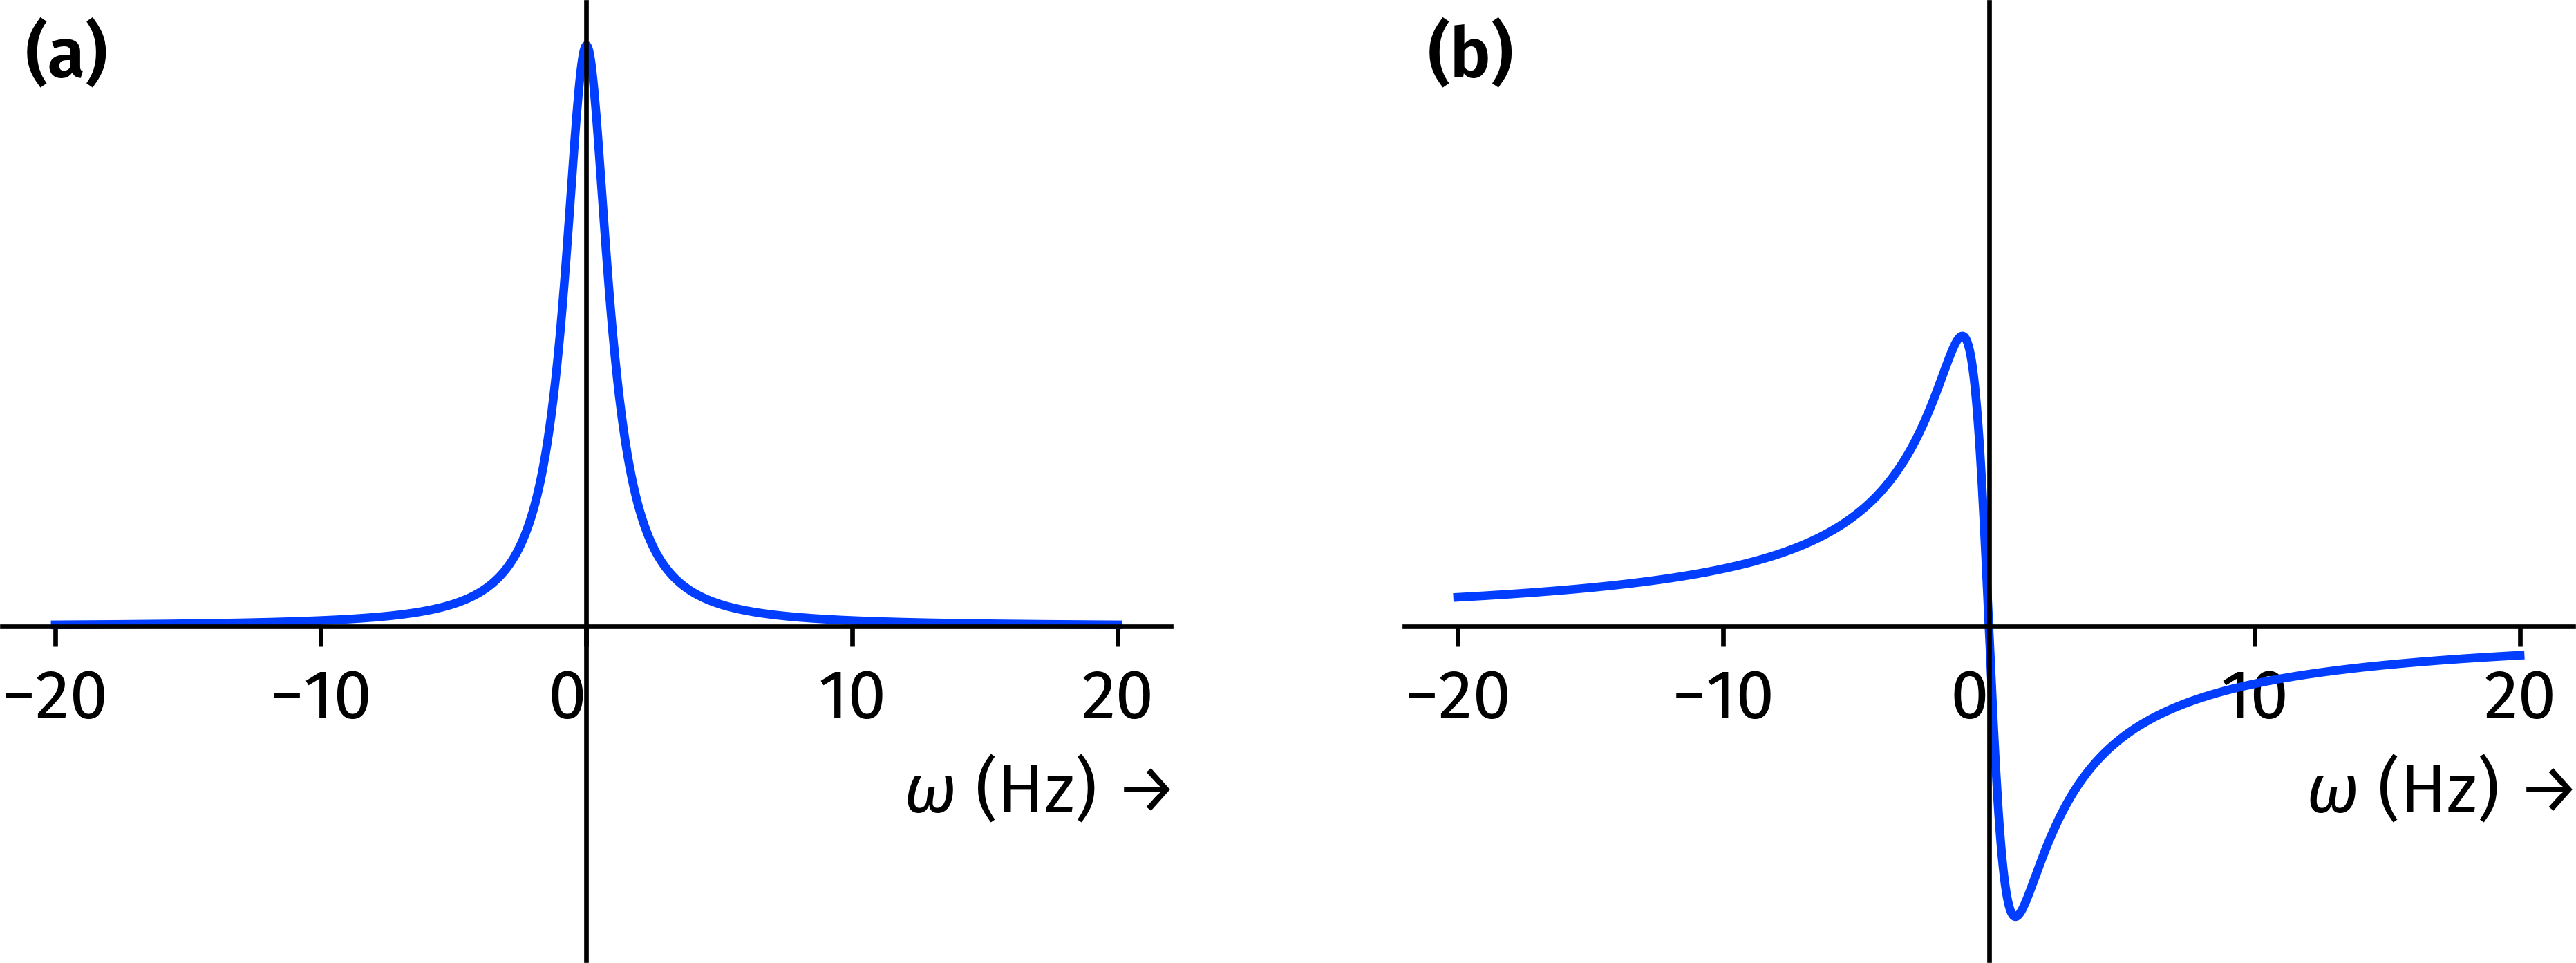
\includegraphics[]{theory/lorentzians.png}%
    {\phantomsubcaption\label{fig:lorentzians_absorption}}%
    {\phantomsubcaption\label{fig:lorentzians_dispersion}}%
    \caption[Absorption- and dispersion-mode Lorentzian lineshapes]{
        \textbf{(\subref{fig:lorentzians_absorption})} Absorption-mode lineshape $A(\omega; \Omega = 0)$.
        \textbf{(\subref{fig:lorentzians_dispersion})} Dispersion-mode lineshape $D(\omega; \Omega = 0)$.
        Both lines have been plotted using $k = \qty{\pi}{\radian\per\second}$.
    }
    \label{fig:lorentzians}
\end{figure}

Strictly speaking, the Lorentzian lineshapes above are only obtained when there is nonzero relaxation during the FID.
For example, in the limit $k \to 0$, $A(\omega; \Omega)$ tends to a delta function $\delta(\omega = \Omega)$.
However, for simplicity, in this thesis I will drop the relaxation term $\exp(-kt)$ unless absolutely necessary; I will simply pretend that a signal of the form $s(t) = \exp(\mi \Omega t)$ is directly Fourier transformed to give $A(\omega; \Omega) + \mi D(\omega; \Omega)$.

Consider now changing the initial pulse such that it is applied along the $+x$-axis instead ($\phi = 0$).
Repeating the above analysis, we find that the resulting signal will have a phase shift:
\begin{align}
    \label{eq:fid_phase_shifted}
    s'(t) &= -\mi\exp(\mi\Omega t) \\
    \Rightarrow \quad S'(\omega) &= \mathcal{F}[s'(t)] = D(\omega;\Omega) - \mi A(\omega;\Omega).
\end{align}
If we were to take the real part of the spectrum here, then we would obtain the undesired dispersion-mode lineshape $D(\omega;\Omega)$.
There are two ways of removing this phase shift.
The first is to shift the \textit{receiver phase} by $\phi_\text{rec}$, which introduces an extra factor of $\exp(-\mi\phi_\text{rec})$ to the detected signal: we can thus choose $\phi_\text{rec} = 3\pi/2$ in order to cancel out the $-\mi$ term in $s'(t)$.
Alternatively, the spectrum can be processed through \textit{phase correction}, in which $S(\omega)$ is directly multiplied by a term $\exp(\mi\phi_\text{corr})$, where $\phi_\text{corr}$ is a linear function of the frequency $\omega$:
\begin{equation}
    \label{eq:phase_correction}
    \phi_\text{corr} = \phi_{\text{corr}}^{(0)} + \omega\phi_{\text{corr}}^{(1)}.
\end{equation}
$\phi_\text{corr}^{(0)}$ and $\phi_\text{corr}^{(1)}$ are respectively termed the \textit{zeroth-} and \textit{first-order phase corrections}: in this idealised case, we can simply choose $(\phi_\text{corr}^{(0)}, \phi_\text{corr}^{(1)}) = (\pi/2, 0)$ to again remove the unwanted phase shift.
More realistically, due to instrumental imperfections, both of these values will have to be nonzero in order to ensure that every peak in the spectrum has the correct phase, i.e.\ is displayed in absorption-mode.

An alternative framework for analysing pulse sequences is to use the ladder operators $I_+$ and $I_-$ (\cref{eq:other_single_spin_ops}).
Using the original example with our initial pulse on $+y$, the density operator immediately after the pulse is:
\begin{equation}
    \label{eq:rho_coherences}
    \rho = I_x = \frac{1}{2}(I_+ + I_-),
\end{equation}
and during detection this evolves as:
\begin{equation}
    \label{eq:fid_coherences}
    \rho(t) = \cos(\Omega t)I_x + \sin(\Omega t)I_y = \frac{1}{2}\left[\exp(-\mi \Omega t)I_+ + \exp(\mi \Omega t)I_- \right].
\end{equation}
(Notice that the $+1$-coherence $I_+$ actually evolves at the negative frequency $-\Omega$.)
To obtain the same signal as previously done in \cref{eq:fid}, we `detect' the $I_-$ term:
\begin{equation}
    \label{eq:detection_coherences}
    s(t) \propto \Tr[I_- \rho(t)] \propto \exp(\mi\Omega t),
\end{equation}
which leads to the common assertion that \textit{only quantum coherences of order $-1$ are detectable}.
It is true that coherences with orders $p = 0, \pm 2, \pm 3, \ldots$ can never be detected in an FID.
However, it is worth pointing out that the `uniqueness' of $-1$-coherence is merely a result of how the $x$- and $y$-magnetisation are combined to form the complex signal (\cref{eq:quadrature}).
We do not \textit{physically} detect $I_-$: we detect $I_x$ and $I_y$, and combine them to form a complex signal which is mathematically equal to detecting $I_-$.
If we had instead chosen to combine them in a different way, such as $s(t) = M_x(t) - \mi M_y(t)$, this would give us $s(t) \propto \exp(-\mi\Omega t)$---corresponding to `detection' of $+1$-coherence---although this alternative does come with the drawback that frequencies must be reversed after Fourier transformation.
In any case, we will stick to the established convention of detecting $-1$-coherence here.

To end this section, it should be pointed out that the complex signal is not obtained as an infinitely-long, continuous function of time, as the treatment above implies.
The complex-valued signal is digitised at an interval called the \textit{dwell time}, $\tau_\text{dw}$, and detection must be stopped after a finite period called the \textit{acquisition time}, $\tau_\text{aq}$.
The FT being performed is actually a discrete Fourier transform (DFT), which yields a periodic function $S(\omega)$; its period (in Hz) is given by $1/\tau_\text{dw}$.%
\footnote{The periodicity property of the DFT is equivalent to the Nyquist theorem, which is usually formulated as follows: the sampling rate required to correctly digitise a signal containing frequencies in the range $[0, f_\text{max}]$ is $1/(2f_\text{max})$. In the main text, it appears as if we have dropped the factor of $2$ in the denominator; but in truth this statement of the Nyquist theorem is applicable to \textit{real-valued} signals, and here we have a \textit{complex-valued} signal $s(t)$, which effectively doubles the range of correctly sampled frequencies.}
The NMR spectrum displayed to the user corresponds to one single period of $S(\omega)$, and thus the \textit{spectral width} is also equal to $1/\tau_\text{dw}$.%
\footnote{Frustratingly, the \texttt{DW} parameter in Bruker's TopSpin software is actually equal to $\tau_\text{dw}/2$. The reason is because this parameter corresponds to the interval between which \textit{real} data is sampled, which is effectively twice as fast as complex-valued sampling.}
In principle, the periodicity of the DFT means that signals which would ordinarily fall outside of the spectral width would appear at incorrect frequencies in the spectrum.\autocite{Turner1986JMR}
On modern instrumentation, this is no longer the case for direct detection; peaks outside of the spectral width are removed using digital filters.
However, \textit{folding} or \textit{aliasing} of peaks in the indirect dimension(s) of multidimensional NMR spectra still occurs.

The DFT $S(\omega)$ is also a discrete function itself, and its resolution is given by $1/\tau_\text{aq}$.
It is possible to extend the effective acquisition time (and thus improve spectral resolution) without actually acquiring more data: this can be done either by \textit{forward linear prediction} of the signal, or by simply adding zeros onto the end of the signal (\textit{zero-filling}).


\subsection{INEPT and product operators}
\label{subsec:theory__inept}

\begin{figure}[htbp]
    \centering
    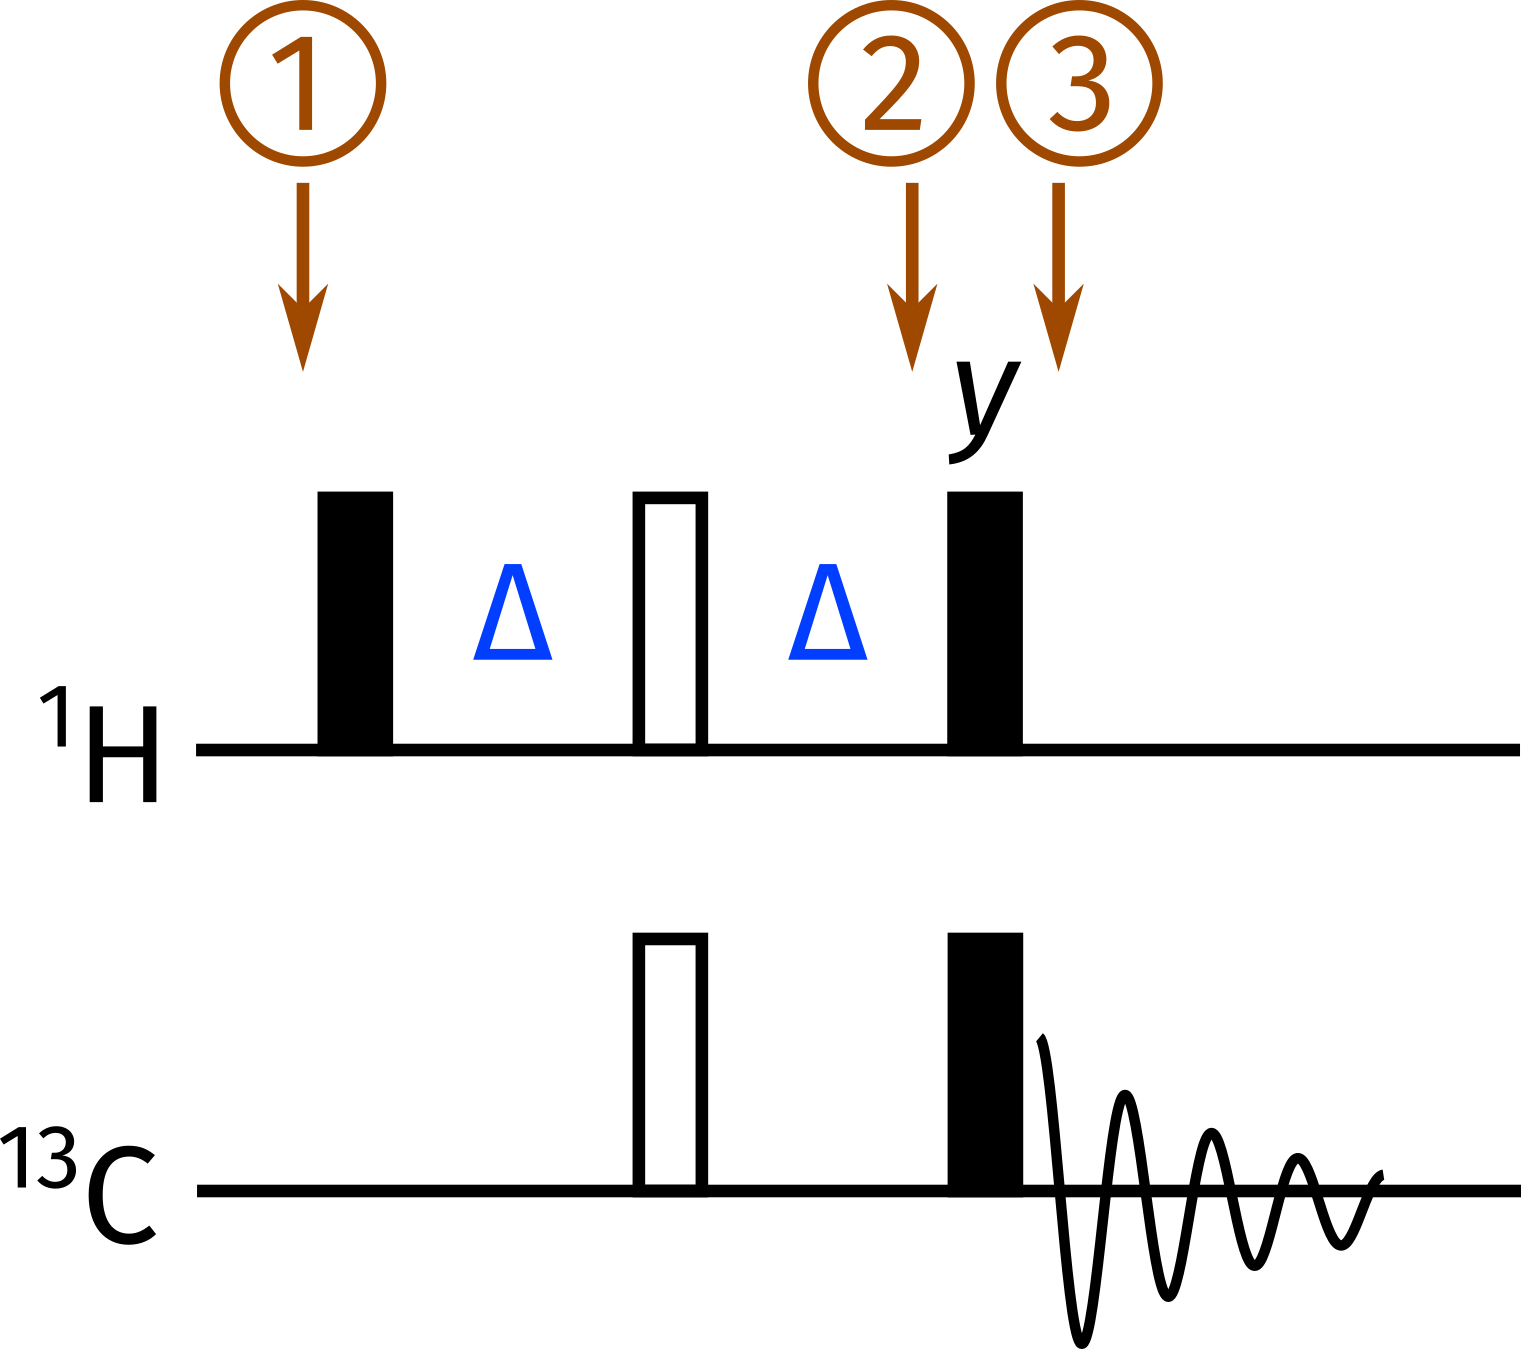
\includegraphics[]{pp/inept.png}%
    \caption[INEPT pulse sequence]{
        INEPT pulse sequence.
        The delay $\Delta$ is set to $1/(4 \cdot \oneJ{CH})$.
    }
    \label{fig:inept}
\end{figure}

Having tackled a simple single-spin case, we now move to the analysis of coupled spin systems and the development of the so-called `product operator formalism'.\autocite{Sorensen1984PNMRS}
In particular, we look at the INEPT experiment\autocite{Morris1979JACS,Morris1980JACS}, in which magnetisation is transferred from a a nuclide with a high magnetogyric ratio to one with a low magnetogyric ratio through a scalar coupling: for example, from \proton{} to \carbon{} using the one-bond coupling constant, $\oneJ{CH}$ (\cref{fig:inept}).
Following tradition, the two nuclei are respectively labelled $I\/$ and $S$.%
\footnote{This may seem insensible since $I\/$ is the \textit{sensitive} and $S$ the \textit{insensitive} nucleus, and indeed, in the original literature\autocite{Morris1979JACS} the meanings of $I\/$ and $S$ were swapped. However, this usage has not been consistent\autocite{Pines1972JCP}, and in modern usage the identification of $I\/$ as the sensitive nucleus seems to have prevailed.}
The Schr\"odinger-picture free Hamiltonian for a weakly coupled system (cf.\ \cref{eq:weak_coupling,eq:h_j_secular}) is $H_\text{free} = \omega_{0,I} I_z + \omega_{0,S} S_z + 2\pi J_{IS} I_z S_z$.
At the very beginning of the sequence (point \circled{1}), we formally have the equilibrium density operator
\begin{equation}
    \label{eq:density_eqm_heteronuclear_full}
    \rho_0 = \frac{\exp(-\beta\hbar H_\text{free})}{\Tr[\exp(-\beta\hbar H_\text{free})]}
    \approx E - \beta\hbar (\omega_{0,I} I_z + \omega_{0,S} S_z + 2\pi J_{IS} I_z S_z),
\end{equation}
using the same approximations as in \cref{eq:nmr_equilibrium_rho}.
The scalar coupling term can be safely neglected as $2\pi J_{IS}$ is several orders of magnitude smaller than the Larmor frequencies $\omega_0$.
After removing the physically irrelevant $E\/$ term and factoring out a constant of $\beta\hbar B_0$, we end up with:
\begin{equation}
    \label{eq:density_eqm_heteronuclear_simplified}
    \rho'_0 = \gamma_I I_z + \gamma_S S_z.
\end{equation}
This represents equilibrium magnetisation (or \textit{polarisation}) on both spins $I\/$ and $S$, in proportion to their magnetogyric ratios.
In general, an NMR experiment may manipulate---and ultimately detect---both of these terms.
Since unitary evolution according to the Liouville--von Neumann equation is \textit{linear}, in that $U(\rho_1 + \rho_2)\adj{U} = U\rho_1\adj{U} + U\rho_2\adj{U}$, we can treat these two terms separately: we focus first on the spin-$I\/$ polarisation, $\rho_I = \gamma_I I_z$.
The first $90^\circ_x$ \proton{} pulse tips this magnetisation into the transverse plane (ignoring off-resonance effects):
\begin{equation}
    \label{eq:rho_after_pulse_x}
    \rho_I \to \exp[-\mi(\pi/2) I_x] \gamma_I I_z \exp[\mi(\pi/2) I_x] = -\gamma_I I_y.
\end{equation}
In principle, we could continue in this manner through repeated application of the `sandwich' formulae (\cref{eq:sandwich_formula_1,eq:sandwich_formula_2}, as well as an analogous version for the $I_zS_z$ term). 
For example, in the $\Delta$ delay which follows, we have that
\begin{equation}
    \label{eq:rho_after_delay_x}
    \begin{aligned}
        \rho_I &\to -\gamma_I\exp(-\mi H_{\text{free},I} \Delta) I_y \exp(\mi H_{\text{free},I} \Delta) \\
               &= -\gamma_I\exp(-\mi H_\text{J} \Delta)\exp(-\mi H_\text{offset}\Delta) I_y \exp(\mi H_\text{offset} \Delta)\exp(\mi H_\text{J}\Delta) \\
               &= \ldots
    \end{aligned}
\end{equation}
When performing simulations of NMR experiments, such as those in later chapters, this is precisely what happens, with the slight difference that the Liouville--von Neumann equation (\cref{eq:lvn_interaction_integrated}) is evaluated numerically rather than symbolically.
Note that in going from the first to the second line, we can only `split up' $H_{\text{free},I}$ into its constituent components $H_\text{offset}$ and $H_\text{J}$ because they commute.

\begin{figure}[htbp]
    \centering
    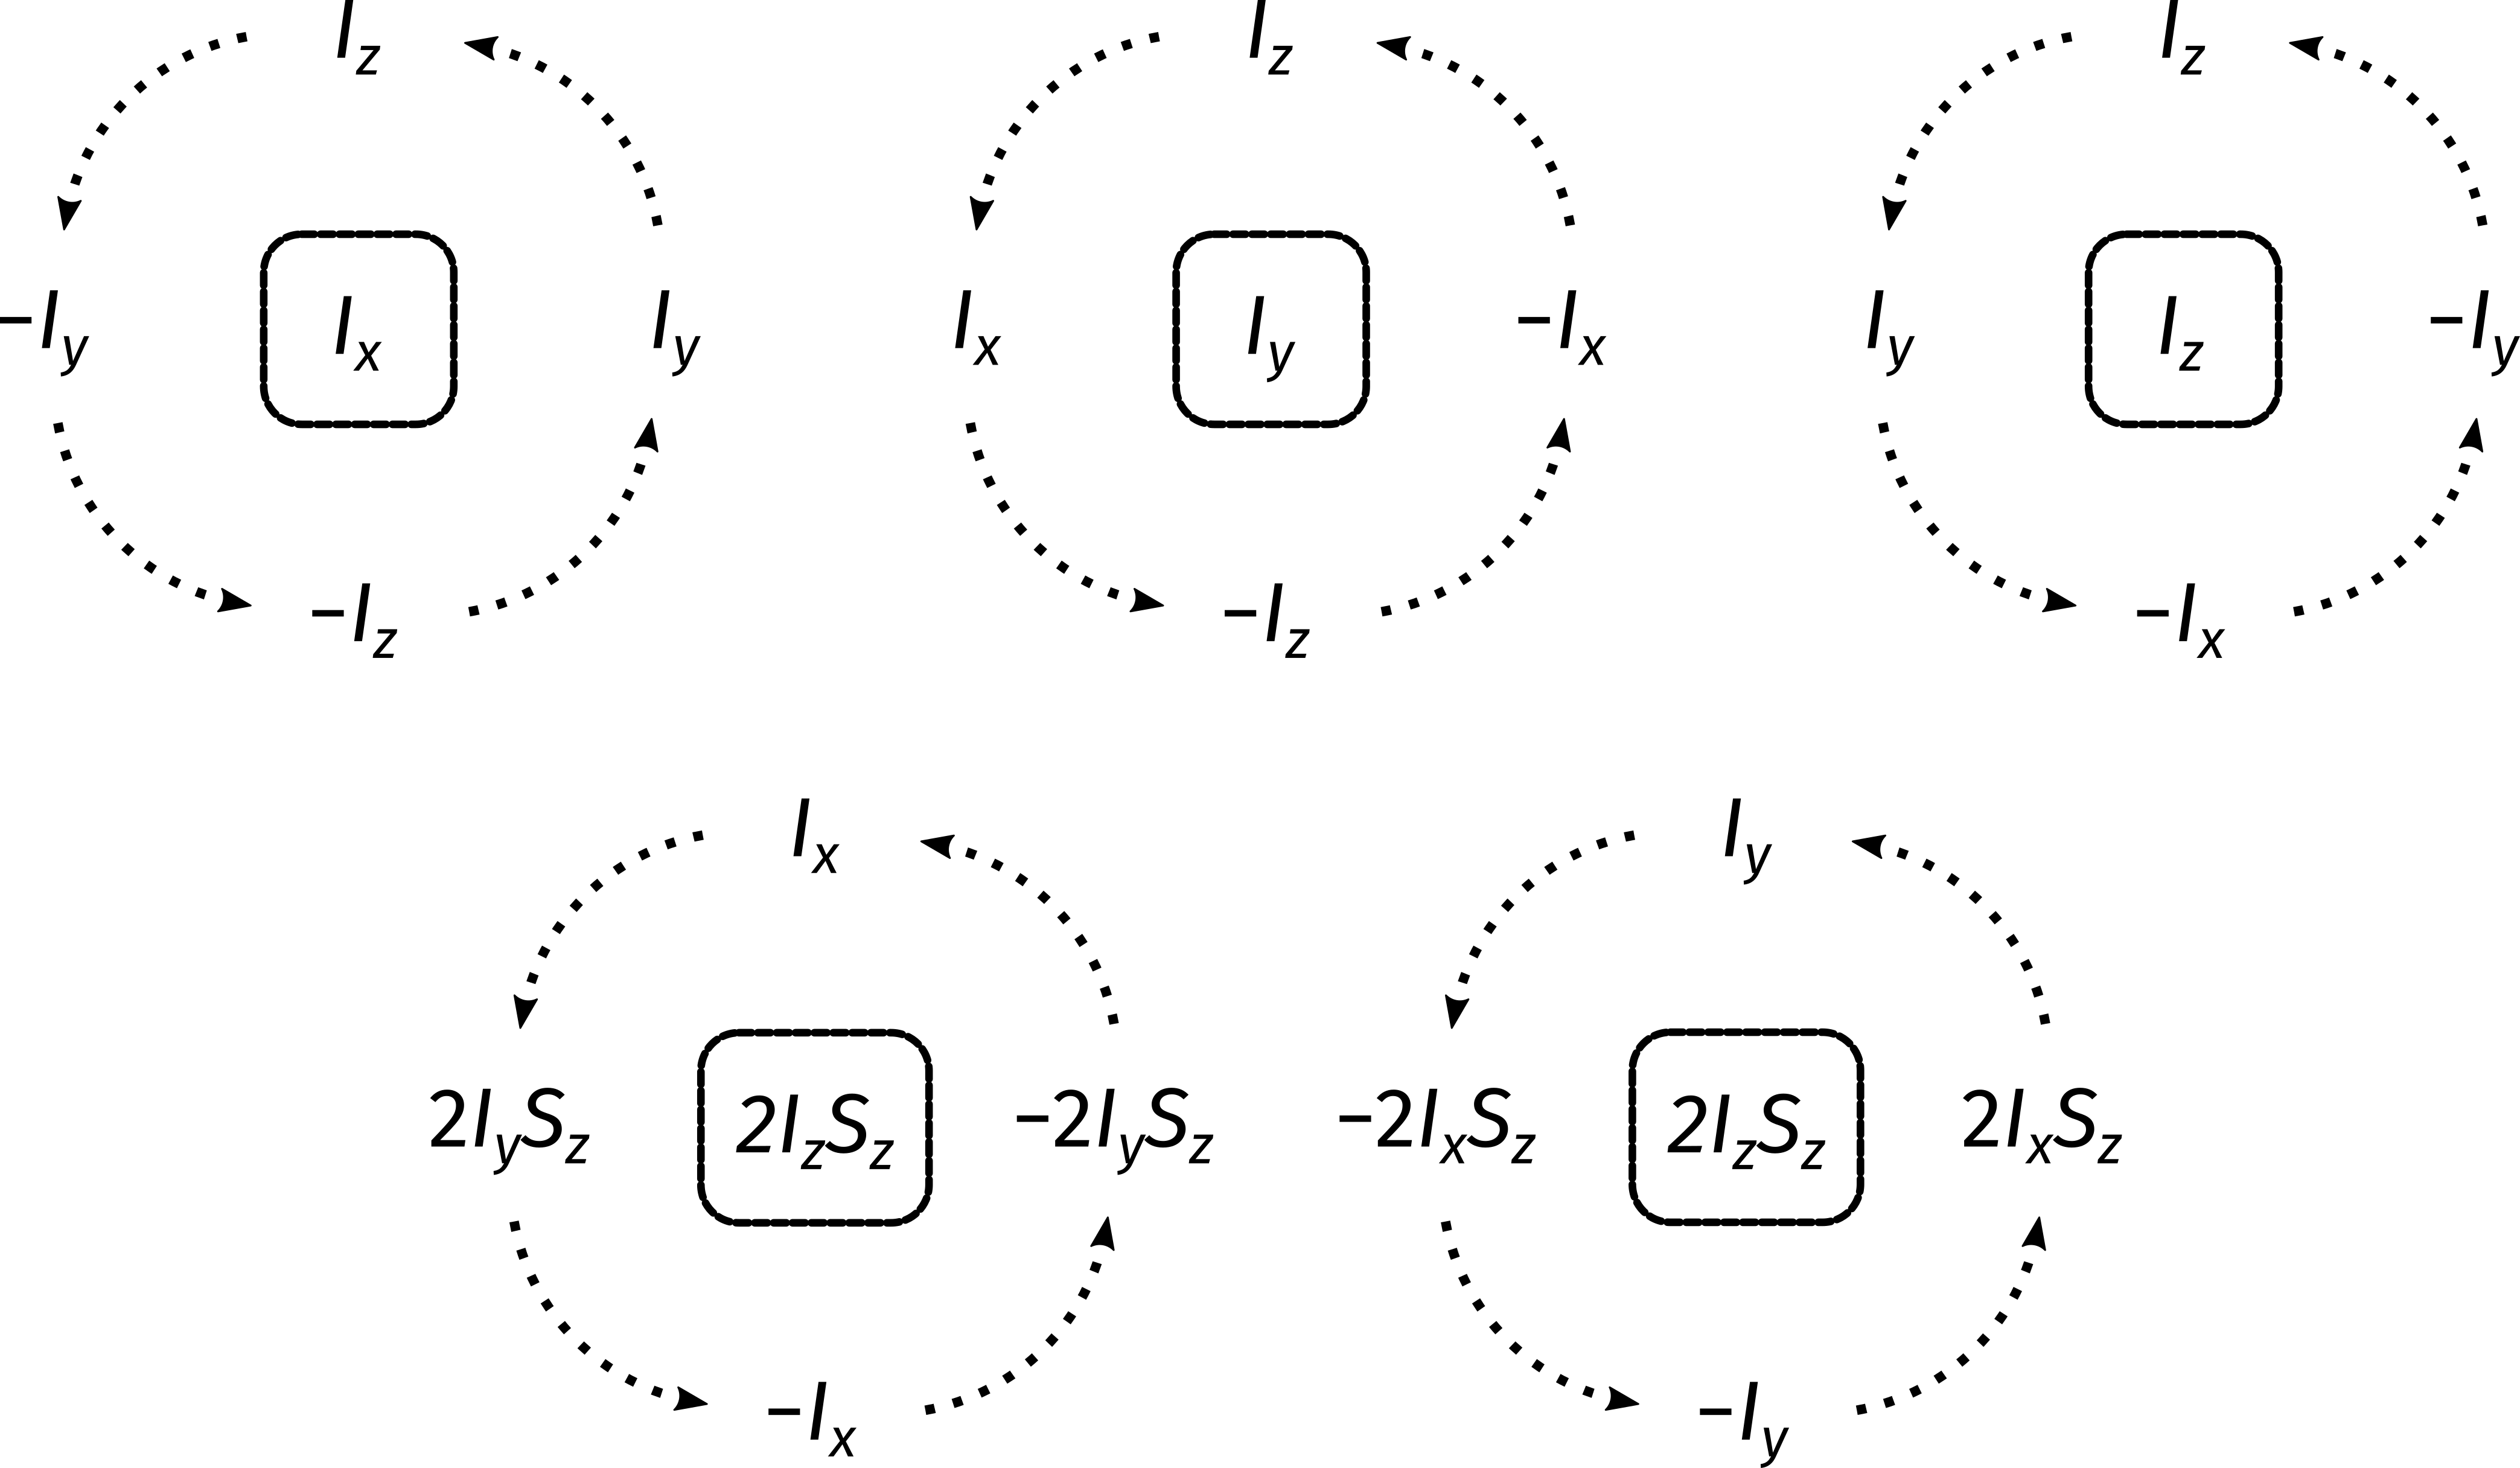
\includegraphics[]{theory/prodop_rules.png}%
    \caption[Simplified rules for product operator evolutions]{
        Simplified rules for the evolution of product operators under different common Hamiltonians (offset, weak/secular J-coupling, and pulses).
        These Hamiltonians often have the form $\omega M$ where $M$ is some `base operator', and are applied for a time $\tau$.
        The boxed operators in the centre of each group refer to $M$; the initial state is then `rotated' about this by an angle of $\omega\tau$ to obtain the final state, or more formally, it is transformed into itself times $\cos(\omega\tau)$, plus the next term in the cycle times $\sin(\omega\tau)$.
        For example, an $90^\circ_x$ pulse has the `base' operator $I_x$ and the angle $\omega\tau = \pi/2$; thus, the initial state $I_z$ would be rotated to $I_z\cos(\pi/2) - I_y\sin(\pi/2) = -I_y$.
    }
    \label{fig:prodop_rules}
\end{figure}

When analysing pulse sequences by hand, however, it is far more convenient to use a set of heuristics which summarise the effects of various pulse sequence elements.
For example, \cref{fig:prodop_rules} summarises the evolution of a density operator under a single term of the Hamiltonian: as above, since $[H_\text{offset}, H_\text{J}] = 0$, we only need to consider one term at a time.
More high-level rules may be devised as well: for example, during the $\Delta\text{--}180^\circ_{x}(I),180^\circ_{x}(S)\text{--}\Delta$ spin echo which comes next, the $J_{IS}$ interaction in $H_{\text{free},I}$ is allowed to evolve for a period of $2\Delta$, but the offset term is \textit{refocused} and can be ignored.
(The sign inversion caused by the \ang{180} pulses must also be included.)
As per \cref{fig:prodop_rules}, this transforms the $-I_y$ term to $-2I_xS_z$ at point \circled{2}: the Hamiltonian is $\pi J_{IS} 2I_zS_z$ for a total time of $2\Delta = 1/(2J_{IS})$, so the `angle' rotated through is $\pi J_{IS}/(2J_{IS}) = \pi/2$.
Immediately after this, the $90^\circ_y(I),90^\circ_x(S)$ pair of pulses rotates this magnetisation to $-2I_zS_y$ (point \circled{3}).
These transformations are often denoted with simpler notation:
\begin{equation}
    \label{eq:inept_prodop}
    \gamma_I I_z
    \xrightarrow{90^\circ_x(I)} -\gamma_I I_y
    \xrightarrow{\Delta\text{--}180^\circ_{x}(I),180^\circ_{x}(S)\text{--}\Delta} -2\gamma_I I_xS_z
    \xrightarrow{90^\circ_y(I),90^\circ_x(S)} -2\gamma_I I_zS_y
\end{equation}
During the detection period, the term $-2\gamma_II_zS_y$ evolves as
\begin{align}
    \label{eq:inept_fid_prodop}
    -2\gamma_I I_zS_y \xrightarrow{H_{\text{free},I}} -2\gamma_I I_zS_y\cos(\Omega_St)\cos(\pi Jt) + \gamma_I S_x\cos(\Omega_St)\sin(\pi Jt) \notag{} \\
    \qquad {} - 2\gamma_I I_zS_x\sin(\Omega_St)\cos(\pi Jt) + \gamma_I S_y\sin(\Omega_S t)\sin(\pi Jt),
\end{align}
from which we extract the complex signal
\begin{equation}
    \label{eq:inept_fid}
    s_I(t) = \langle S_x(t) \rangle + \mi \langle S_y(t) \rangle = \frac{\gamma_I}{2\mi}\bigl\{\exp[\mi(\Omega_S + \pi J_{IS})t] - \exp[\mi(\Omega_S - \pi J_{IS})t]\bigr\}.
\end{equation}
After Fourier transformation, the resulting spectrum has two peaks with opposite phase and have the frequencies $\Omega_S \pm \pi J_{IS}$; because of the factor of $1/(2\mi)$, the real part of the spectrum will contain dispersion-mode signals (\cref{fig:doublet_lorentzians_dis_anti}).
If desired, zeroth-order phase correction can be performed here, yielding instead a pair of absorption-mode signals still with opposite phases (\cref{fig:doublet_lorentzians_abs_anti}).
In either case, this is termed an \textit{antiphase} doublet; the product operators which give rise to it ($2I_zS_x$ and $2I_zS_y$) are said to be antiphase with respect to spin $I\/$.
Importantly, the amplitude of the signal scales as $\gamma_I$ rather than $\gamma_S$; since $\gamma_I > \gamma_S$, this represents a sensitivity enhancement compared to the direct excitation of $S$-magnetisation.

\begin{figure}[htbp]
    \centering
    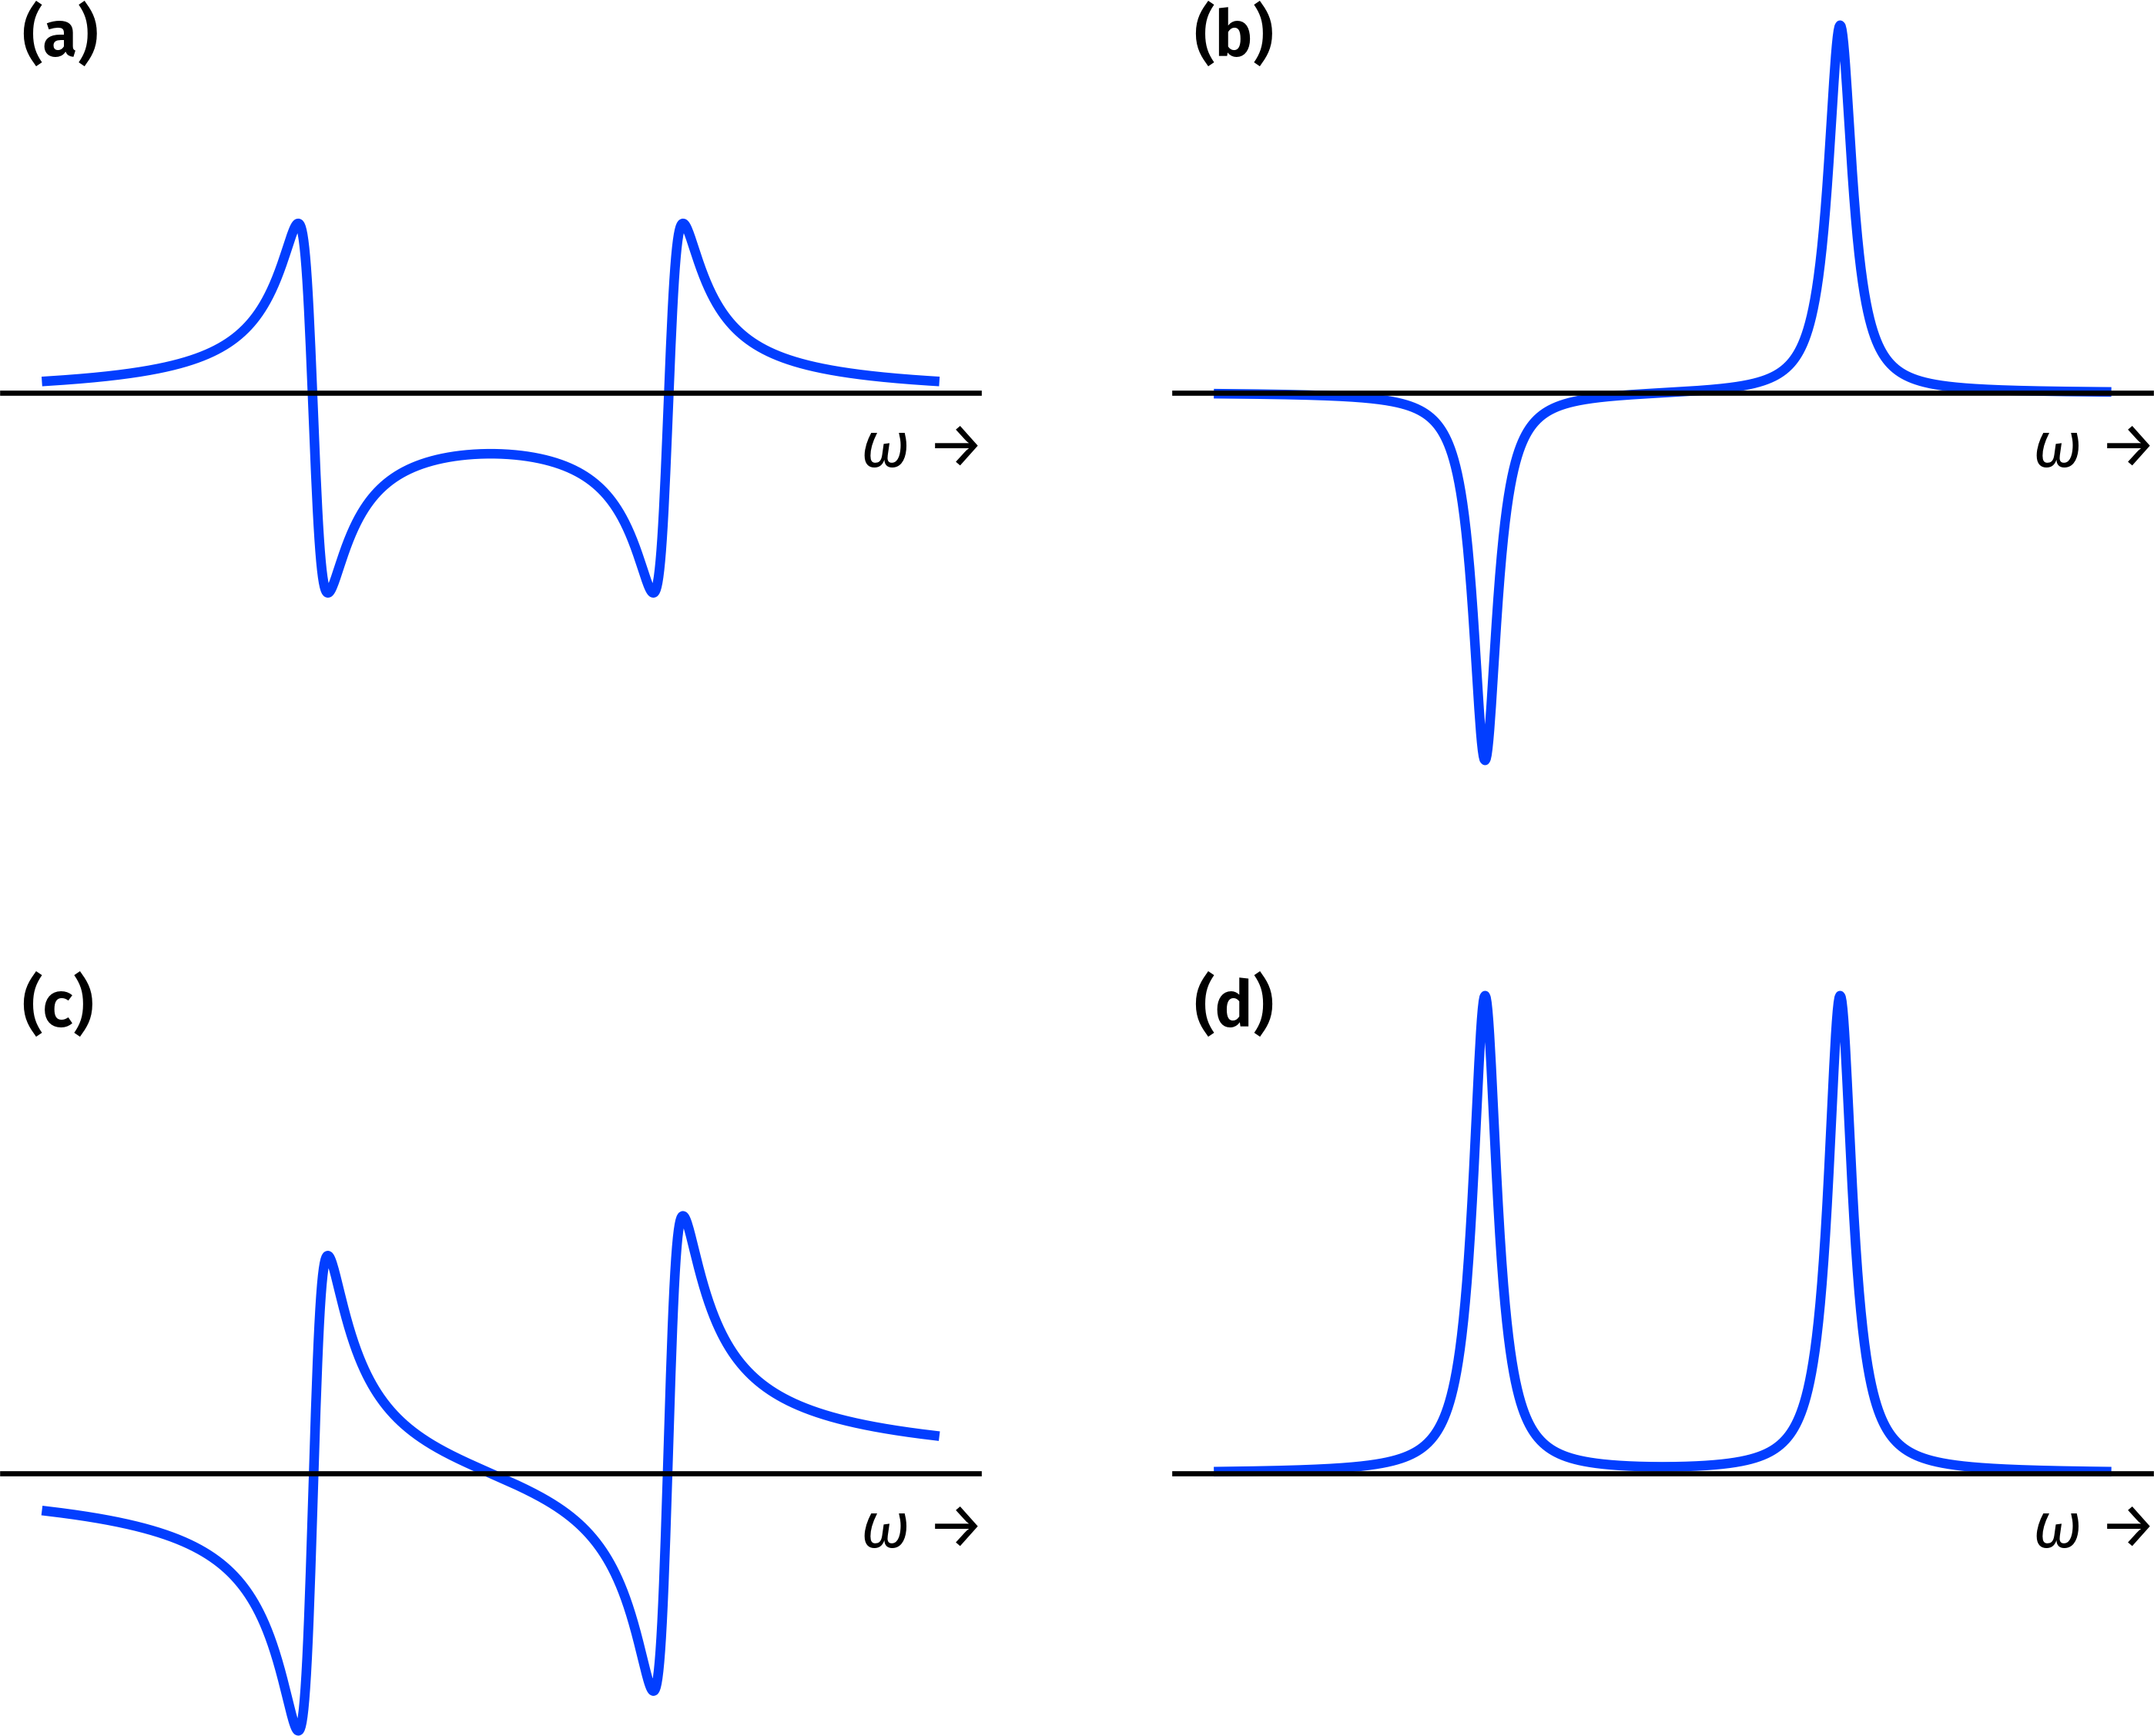
\includegraphics[]{theory/doublet_lorentzians.png}%
    {\phantomsubcaption\label{fig:doublet_lorentzians_dis_anti}}%
    {\phantomsubcaption\label{fig:doublet_lorentzians_abs_anti}}%
    {\phantomsubcaption\label{fig:doublet_lorentzians_dis_in}}%
    {\phantomsubcaption\label{fig:doublet_lorentzians_abs_in}}%
    \caption[Absorption- and dispersion-mode in-phase and antiphase doublets]{
        Peak shapes of a doublet.
        In all cases, the separation between the two peaks is $2\pi J_{IS}$.
        \textbf{(\subref*{fig:doublet_lorentzians_dis_anti})} Antiphase, dispersion-mode.
        \textbf{(\subref*{fig:doublet_lorentzians_abs_anti})} Antiphase, absorption-mode.
        \textbf{(\subref*{fig:doublet_lorentzians_dis_in})} In-phase, dispersion-mode.
        \textbf{(\subref*{fig:doublet_lorentzians_abs_in})} In-phase, absorption-mode.
    }
    \label{fig:doublet_lorentzians}
\end{figure}

Of course, this is only half of the picture; we have not considered what happens to the other part of the magnetisation, namely $\rho_S = \gamma_S S_z$.
Clearly, this is unaffected by the initial $90^\circ_x(I)$ pulse and the first $\Delta$ delay.
The $180^\circ_x(S)$ pulse inverts it, and the final $90^\circ_x(S)$ pulse in fact transforms it into observable $S$-magnetisation:
\begin{equation}
    \label{eq:inept_prodop_s}
    \gamma_S S_z \xrightarrow{90^\circ_x(I)\text{--}\Delta} \gamma_S S_z
    \xrightarrow{180^\circ_x(I),180^\circ_x(S)\text{--}\Delta} -\gamma_S S_z
    \xrightarrow{90^\circ_y(I),90^\circ_x(S)} \gamma_S S_y
\end{equation}
This term produces \textit{in-phase} spin-$S$ magnetisation during the detection period (where the two components of the doublet have the same phase):
\begin{equation}
    \label{eq:inept_fid_S}
    s_S(t) = \frac{\mi\gamma_S}{2}\bigl\{\exp[\mi(\Omega_S + \pi J_{IS})t] + \exp[\mi(\Omega_S - \pi J_{IS})t]\bigr\},
\end{equation}
Because of the factor of $\mi$, the real part of the spectrum will contain a dispersion-mode doublet (\cref{fig:doublet_lorentzians_dis_in}).
The signal actually measured by the spectrometer is $s(t) = s_I(t) + s_S(t)$; and the spectrum is a weighted sum of in-phase and antiphase magnetisation.
This leads to potentially unwanted phase distortions in the spectrum, which one would prefer to suppress.

This can be accomplished through the technique of \textit{phase cycling}, where pulse and receiver phases are changed in concert and the resulting FIDs summed in order to select for a particular signal.
In this case, the INEPT experiment is performed twice, once with the phases as given in \cref{fig:inept}, and once where the initial $90^\circ_x(I)$ pulse is replaced with a $90^\circ_{-x}(I)$ pulse.
The first of these gives us the same signals as above.
However, inverting the initial $I\/$ pulse leads to $s_I$ acquiring a minus sign, because the initial $I_z$ term is rotated to $I_y$ instead of $-I_y$.
On the other hand, the signal component $s_S$ is unaffected by this pulse and thus does not experience a change of sign.
The two FIDs we record are thus as follows:
\begin{align}
    \label{eq:inept_phase_cycling}
    s_1(t) &= s_I(t) + s_S(t) \\
    s_2(t) &= -s_I(t) + s_S(t)
\end{align}
Simply taking the difference of these two FIDs yields a signal where the desired $s_I$ has been accumulated and $s_S$ has been cancelled out.
In practice, instead of subtracting the two signals, it is typical to shift the receiver phase $\phi_\text{rec}$ by \ang{180} in the second experiment: this introduces a phase shift of $\exp(-\mi\pi) = -1$ to the signal, and the two signals can now be \textit{added} together instead of subtracted to cancel out $s_S$.
Since both $\phi_1$ and $\phi_\text{rec}$ are $0$ on the first experiment and $\pi$ on the second experiment, we can express this as $\phi_x = \phi_\text{rec} = (0, \pi)$.
This is more commonly denoted as $\phi_1 = \phi_\text{rec} = (x, -x)$, because the phases $(0, \pi)$ correspond to the $+x$- and $-x$-axes respectively.

The `simplified' analysis of pulse sequences shown in \cref{eq:inept_prodop,eq:inept_prodop_s} is often called \textit{`product operator'} analysis\autocite{Sorensen1984PNMRS}, because the underlying two-spin operators are products of single-spin Cartesian operators.
Although this is often touted as being `simpler' than full density operator calculations, it is really just a shorthand which masks the quantum mechanical theory developed in this chapter:
\begin{equation}
    \label{eq:product_operator_shorthand}
    \underbrace{I_z \xrightarrow{90^\circ_x(I)} -I_y}_{\textit{product operator}}
    \quad\Longleftrightarrow\quad
    \underbrace{\exp(-\mi I_x\pi/2)I_z\exp(\mi I_x\pi/2) = -I_y}_{\textit{density operator}}
\end{equation}
Since the operators $\{E, I_x, I_y, I_z\}$ form a complete basis for a single-spin system, their products (i.e.\ product operators) likewise form a complete basis for multiple-spin systems, and so \textit{any} density matrix for a multiple-spin system may be expressed as a linear combination of product operators.
Strictly speaking, the use of product operators therefore does not actually sacrifice any power in and of itself.
However, the heuristics such as those in \cref{fig:prodop_rules} \textit{are} limiting, in that the evolution under some Hamiltonians---for example, strong coupling $\symbf{I}\cdot\symbf{S}$, or pulses for off-resonance spins where $H\/$ is a sum of $I_x$ and $I_z$---cannot be neatly captured in such a pictorial form.


\subsection{2D NMR: HSQC}
\label{subsec:theory__hsqc}

The use of coherence orders is particularly effective in the analysis of modern 2D NMR experiments, which make use of multiple different techniques to select for particular \textit{coherence transfer pathways} (CTPs).
A full discussion of this is beyond the scope of this thesis.
Nevertheless, the analysis of a 2D \proton{}--\carbon{} HSQC experiment (\cref{fig:hsqc_1grad}) is given here as an example to illustrate the concepts of CTP selection through \textit{phase cycling} and gradients, as well as the related issue of quadrature detection in indirect dimensions.

\begin{figure}[ht]
    \centering
    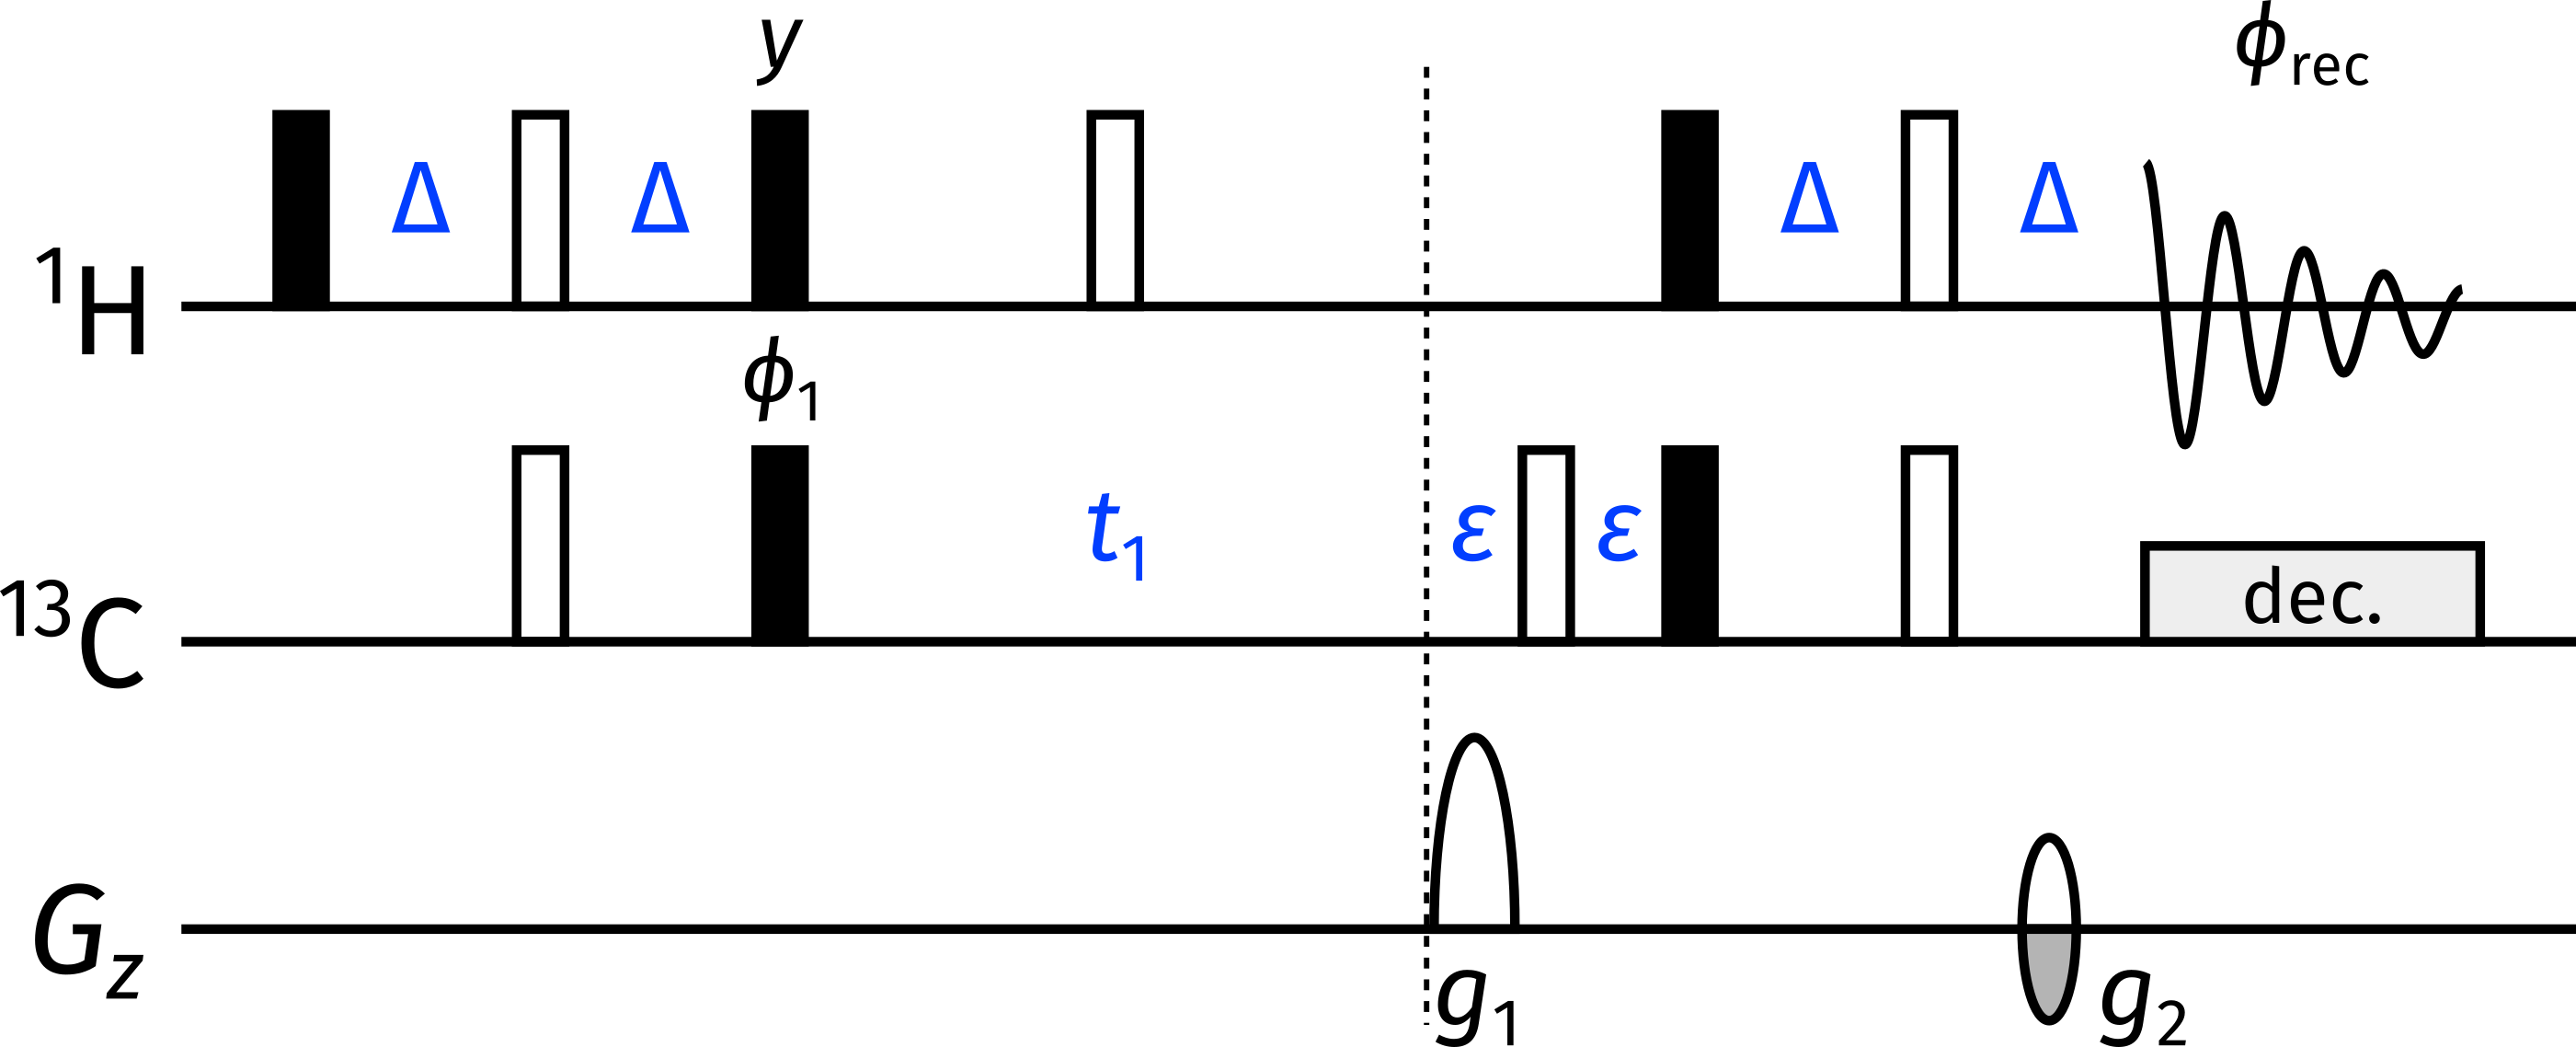
\includegraphics[scale=1.2]{pp/hsqc/hsqc_1grad.png}
    \caption[Echo--antiecho HSQC pulse sequence]{
        A typical echo--antiecho HSQC pulse sequence (the symbols are explained in the \textit{Preface}).
        The pulse phase $\phi_1$ and the receiver phase $\phi_\text{rec}$ are together alternated between $0$ and $\pi$; this is typically denoted as $\phi_1 = \phi_\text{rec} = (x, -x)$ as these phases correspond to the $+x$- and $-x$-axes.
        The delay $\Delta$ is set to $1/(4 \cdot \oneJ{CH})$.
        The gradient amplitudes are chosen such that $|g_1/g_2| = \gamma_{\ch{H}}/\gamma_{\ch{C}} \approx 4$.
        Echo--antiecho CTP selection is carried out by inverting the sign of $g_2$.
    }
    \label{fig:hsqc_1grad}
\end{figure}

The HSQC experiment seeks to only detect protons directly bonded to \carbon{}; all other protons must be suppressed.
We first show how pulsed field gradients and phase cycling allow the \textit{desired} signal to be obtained.

\todo{
This is technically only appropriate for an isolated methine (i.e. \ch{CH}) group.
The analysis which proceeds, however, is identical for methylene and methyl groups, which would be $I_2S$ and $I_3S$ systems respectively.
More unsound is the complete neglect of \ch{H}--\ch{H} coupling.
Luckily, this does not pose a serious problem here: it essentially leads to a small loss of signal.
However, for other experiments it may be necessary to account for $\nJ{HH}$: for example, it causes artefacts in the sensitivity-enhanced HSQC, as will be discussed in \cref{subsec:noah__sehsqc}.
In general, this illustrates the point that one should choose the \textit{simplest possible system} (but not one any simpler) to analyse a pulse sequence.
}


\todo{
\begin{itemize}
    \item CTP selection through gradients, mathematical requirement for CTP to be refocused
    \item Quadrature detection in $F_1$ (ugh)
    \item Composite coherence order\autocite{John1991JMR,Mitschang1995JCP}
    \item phase cycling to cancellation of unwanted peaks (e.g.\ arising from \ch{^{12}C}-bound \ch{^{1}H})
    \item explain why phase cycling (on its own) isn't really used for CTP selection any more
\end{itemize}
}


